% Created by tikzDevice version 0.10.1 on 2017-11-15 12:08:02
% !TEX encoding = UTF-8 Unicode
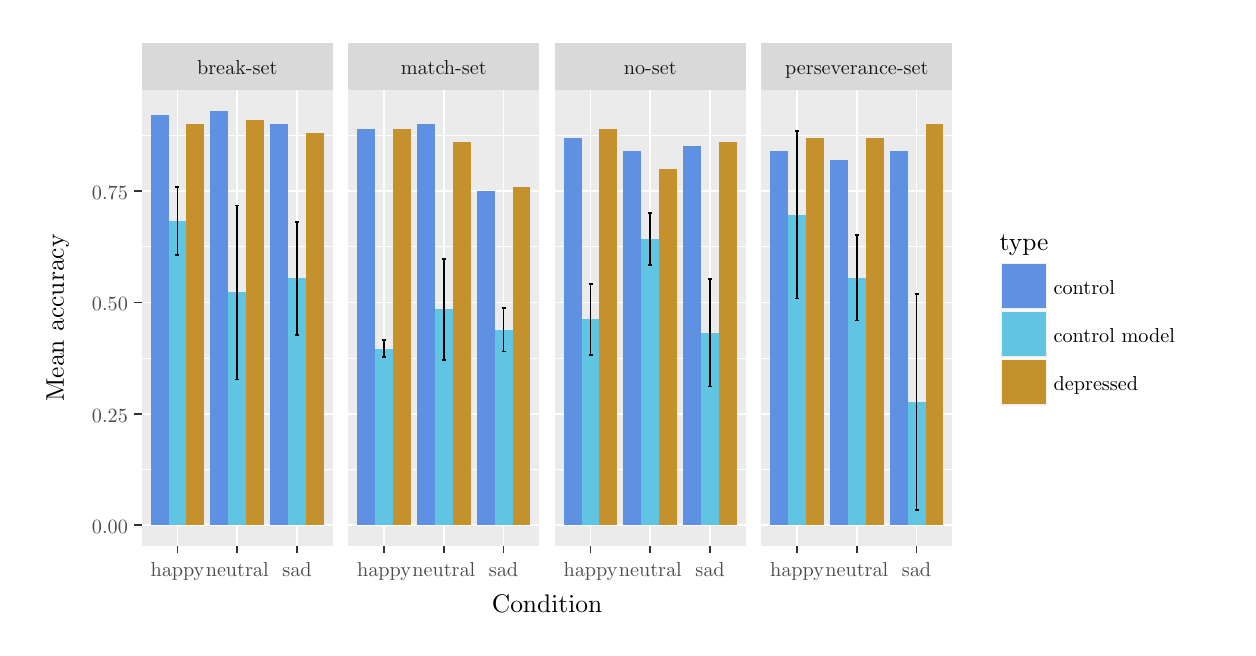
\begin{tikzpicture}[x=1pt,y=1pt]
\definecolor{fillColor}{RGB}{255,255,255}
\path[use as bounding box,fill=fillColor,fill opacity=0.00] (0,0) rectangle (433.62,216.81);
\begin{scope}
\path[clip] (  0.00,  0.00) rectangle (433.62,216.81);
\definecolor{drawColor}{RGB}{255,255,255}
\definecolor{fillColor}{RGB}{255,255,255}

\path[draw=drawColor,line width= 0.6pt,line join=round,line cap=round,fill=fillColor] (  0.00,  0.00) rectangle (433.62,216.81);
\end{scope}
\begin{scope}
\path[clip] ( 41.17, 29.59) rectangle (110.29,194.25);
\definecolor{fillColor}{gray}{0.92}

\path[fill=fillColor] ( 41.17, 29.59) rectangle (110.29,194.25);
\definecolor{drawColor}{RGB}{255,255,255}

\path[draw=drawColor,line width= 0.3pt,line join=round] ( 41.17, 57.19) --
	(110.29, 57.19);

\path[draw=drawColor,line width= 0.3pt,line join=round] ( 41.17, 97.43) --
	(110.29, 97.43);

\path[draw=drawColor,line width= 0.3pt,line join=round] ( 41.17,137.67) --
	(110.29,137.67);

\path[draw=drawColor,line width= 0.3pt,line join=round] ( 41.17,177.91) --
	(110.29,177.91);

\path[draw=drawColor,line width= 0.6pt,line join=round] ( 41.17, 37.07) --
	(110.29, 37.07);

\path[draw=drawColor,line width= 0.6pt,line join=round] ( 41.17, 77.31) --
	(110.29, 77.31);

\path[draw=drawColor,line width= 0.6pt,line join=round] ( 41.17,117.55) --
	(110.29,117.55);

\path[draw=drawColor,line width= 0.6pt,line join=round] ( 41.17,157.79) --
	(110.29,157.79);

\path[draw=drawColor,line width= 0.6pt,line join=round] ( 54.13, 29.59) --
	( 54.13,194.25);

\path[draw=drawColor,line width= 0.6pt,line join=round] ( 75.73, 29.59) --
	( 75.73,194.25);

\path[draw=drawColor,line width= 0.6pt,line join=round] ( 97.33, 29.59) --
	( 97.33,194.25);
\definecolor{fillColor}{RGB}{196,145,45}

\path[fill=fillColor] ( 57.37, 37.07) rectangle ( 63.85,181.94);
\definecolor{fillColor}{RGB}{95,197,226}

\path[fill=fillColor] ( 50.89, 37.07) rectangle ( 57.37,147.06);
\definecolor{fillColor}{RGB}{95,145,226}

\path[fill=fillColor] ( 44.41, 37.07) rectangle ( 50.89,185.16);
\definecolor{fillColor}{RGB}{196,145,45}

\path[fill=fillColor] ( 78.97, 37.07) rectangle ( 85.45,183.55);
\definecolor{fillColor}{RGB}{95,197,226}

\path[fill=fillColor] ( 72.49, 37.07) rectangle ( 78.97,121.13);
\definecolor{fillColor}{RGB}{95,145,226}

\path[fill=fillColor] ( 66.01, 37.07) rectangle ( 72.49,186.76);
\definecolor{fillColor}{RGB}{196,145,45}

\path[fill=fillColor] (100.57, 37.07) rectangle (107.05,178.72);
\definecolor{fillColor}{RGB}{95,197,226}

\path[fill=fillColor] ( 94.09, 37.07) rectangle (100.57,126.26);
\definecolor{fillColor}{RGB}{95,145,226}

\path[fill=fillColor] ( 87.61, 37.07) rectangle ( 94.09,181.94);
\definecolor{drawColor}{RGB}{0,0,0}

\path[draw=drawColor,line width= 0.6pt,line join=round] ( 53.41,159.35) --
	( 54.85,159.35);

\path[draw=drawColor,line width= 0.6pt,line join=round] ( 54.13,159.35) --
	( 54.13,134.77);

\path[draw=drawColor,line width= 0.6pt,line join=round] ( 53.41,134.77) --
	( 54.85,134.77);

\path[draw=drawColor,line width= 0.6pt,line join=round] ( 75.01,152.57) --
	( 76.45,152.57);

\path[draw=drawColor,line width= 0.6pt,line join=round] ( 75.73,152.57) --
	( 75.73, 89.69);

\path[draw=drawColor,line width= 0.6pt,line join=round] ( 75.01, 89.69) --
	( 76.45, 89.69);

\path[draw=drawColor,line width= 0.6pt,line join=round] ( 96.61,146.67) --
	( 98.05,146.67);

\path[draw=drawColor,line width= 0.6pt,line join=round] ( 97.33,146.67) --
	( 97.33,105.84);

\path[draw=drawColor,line width= 0.6pt,line join=round] ( 96.61,105.84) --
	( 98.05,105.84);
\end{scope}
\begin{scope}
\path[clip] (115.79, 29.59) rectangle (184.92,194.25);
\definecolor{fillColor}{gray}{0.92}

\path[fill=fillColor] (115.79, 29.59) rectangle (184.92,194.25);
\definecolor{drawColor}{RGB}{255,255,255}

\path[draw=drawColor,line width= 0.3pt,line join=round] (115.79, 57.19) --
	(184.92, 57.19);

\path[draw=drawColor,line width= 0.3pt,line join=round] (115.79, 97.43) --
	(184.92, 97.43);

\path[draw=drawColor,line width= 0.3pt,line join=round] (115.79,137.67) --
	(184.92,137.67);

\path[draw=drawColor,line width= 0.3pt,line join=round] (115.79,177.91) --
	(184.92,177.91);

\path[draw=drawColor,line width= 0.6pt,line join=round] (115.79, 37.07) --
	(184.92, 37.07);

\path[draw=drawColor,line width= 0.6pt,line join=round] (115.79, 77.31) --
	(184.92, 77.31);

\path[draw=drawColor,line width= 0.6pt,line join=round] (115.79,117.55) --
	(184.92,117.55);

\path[draw=drawColor,line width= 0.6pt,line join=round] (115.79,157.79) --
	(184.92,157.79);

\path[draw=drawColor,line width= 0.6pt,line join=round] (128.76, 29.59) --
	(128.76,194.25);

\path[draw=drawColor,line width= 0.6pt,line join=round] (150.36, 29.59) --
	(150.36,194.25);

\path[draw=drawColor,line width= 0.6pt,line join=round] (171.96, 29.59) --
	(171.96,194.25);
\definecolor{fillColor}{RGB}{196,145,45}

\path[fill=fillColor] (132.00, 37.07) rectangle (138.48,180.33);
\definecolor{fillColor}{RGB}{95,197,226}

\path[fill=fillColor] (125.51, 37.07) rectangle (132.00,100.85);
\definecolor{fillColor}{RGB}{95,145,226}

\path[fill=fillColor] (119.03, 37.07) rectangle (125.51,180.33);
\definecolor{fillColor}{RGB}{196,145,45}

\path[fill=fillColor] (153.60, 37.07) rectangle (160.08,175.50);
\definecolor{fillColor}{RGB}{95,197,226}

\path[fill=fillColor] (147.12, 37.07) rectangle (153.60,115.02);
\definecolor{fillColor}{RGB}{95,145,226}

\path[fill=fillColor] (140.64, 37.07) rectangle (147.12,181.94);
\definecolor{fillColor}{RGB}{196,145,45}

\path[fill=fillColor] (175.20, 37.07) rectangle (181.68,159.40);
\definecolor{fillColor}{RGB}{95,197,226}

\path[fill=fillColor] (168.72, 37.07) rectangle (175.20,107.70);
\definecolor{fillColor}{RGB}{95,145,226}

\path[fill=fillColor] (162.24, 37.07) rectangle (168.72,157.79);
\definecolor{drawColor}{RGB}{0,0,0}

\path[draw=drawColor,line width= 0.6pt,line join=round] (128.04,104.02) --
	(129.48,104.02);

\path[draw=drawColor,line width= 0.6pt,line join=round] (128.76,104.02) --
	(128.76, 97.69);

\path[draw=drawColor,line width= 0.6pt,line join=round] (128.04, 97.69) --
	(129.48, 97.69);

\path[draw=drawColor,line width= 0.6pt,line join=round] (149.64,133.24) --
	(151.08,133.24);

\path[draw=drawColor,line width= 0.6pt,line join=round] (150.36,133.24) --
	(150.36, 96.81);

\path[draw=drawColor,line width= 0.6pt,line join=round] (149.64, 96.81) --
	(151.08, 96.81);

\path[draw=drawColor,line width= 0.6pt,line join=round] (171.24,115.61) --
	(172.68,115.61);

\path[draw=drawColor,line width= 0.6pt,line join=round] (171.96,115.61) --
	(171.96, 99.79);

\path[draw=drawColor,line width= 0.6pt,line join=round] (171.24, 99.79) --
	(172.68, 99.79);
\end{scope}
\begin{scope}
\path[clip] (190.42, 29.59) rectangle (259.54,194.25);
\definecolor{fillColor}{gray}{0.92}

\path[fill=fillColor] (190.42, 29.59) rectangle (259.54,194.25);
\definecolor{drawColor}{RGB}{255,255,255}

\path[draw=drawColor,line width= 0.3pt,line join=round] (190.42, 57.19) --
	(259.54, 57.19);

\path[draw=drawColor,line width= 0.3pt,line join=round] (190.42, 97.43) --
	(259.54, 97.43);

\path[draw=drawColor,line width= 0.3pt,line join=round] (190.42,137.67) --
	(259.54,137.67);

\path[draw=drawColor,line width= 0.3pt,line join=round] (190.42,177.91) --
	(259.54,177.91);

\path[draw=drawColor,line width= 0.6pt,line join=round] (190.42, 37.07) --
	(259.54, 37.07);

\path[draw=drawColor,line width= 0.6pt,line join=round] (190.42, 77.31) --
	(259.54, 77.31);

\path[draw=drawColor,line width= 0.6pt,line join=round] (190.42,117.55) --
	(259.54,117.55);

\path[draw=drawColor,line width= 0.6pt,line join=round] (190.42,157.79) --
	(259.54,157.79);

\path[draw=drawColor,line width= 0.6pt,line join=round] (203.38, 29.59) --
	(203.38,194.25);

\path[draw=drawColor,line width= 0.6pt,line join=round] (224.98, 29.59) --
	(224.98,194.25);

\path[draw=drawColor,line width= 0.6pt,line join=round] (246.58, 29.59) --
	(246.58,194.25);
\definecolor{fillColor}{RGB}{196,145,45}

\path[fill=fillColor] (206.62, 37.07) rectangle (213.10,180.33);
\definecolor{fillColor}{RGB}{95,197,226}

\path[fill=fillColor] (200.14, 37.07) rectangle (206.62,111.36);
\definecolor{fillColor}{RGB}{95,145,226}

\path[fill=fillColor] (193.66, 37.07) rectangle (200.14,177.11);
\definecolor{fillColor}{RGB}{196,145,45}

\path[fill=fillColor] (228.22, 37.07) rectangle (234.70,165.84);
\definecolor{fillColor}{RGB}{95,197,226}

\path[fill=fillColor] (221.74, 37.07) rectangle (228.22,140.42);
\definecolor{fillColor}{RGB}{95,145,226}

\path[fill=fillColor] (215.26, 37.07) rectangle (221.74,172.28);
\definecolor{fillColor}{RGB}{196,145,45}

\path[fill=fillColor] (249.82, 37.07) rectangle (256.30,175.50);
\definecolor{fillColor}{RGB}{95,197,226}

\path[fill=fillColor] (243.34, 37.07) rectangle (249.82,106.62);
\definecolor{fillColor}{RGB}{95,145,226}

\path[fill=fillColor] (236.86, 37.07) rectangle (243.34,173.89);
\definecolor{drawColor}{RGB}{0,0,0}

\path[draw=drawColor,line width= 0.6pt,line join=round] (202.66,124.26) --
	(204.10,124.26);

\path[draw=drawColor,line width= 0.6pt,line join=round] (203.38,124.26) --
	(203.38, 98.45);

\path[draw=drawColor,line width= 0.6pt,line join=round] (202.66, 98.45) --
	(204.10, 98.45);

\path[draw=drawColor,line width= 0.6pt,line join=round] (224.26,149.81) --
	(225.70,149.81);

\path[draw=drawColor,line width= 0.6pt,line join=round] (224.98,149.81) --
	(224.98,131.03);

\path[draw=drawColor,line width= 0.6pt,line join=round] (224.26,131.03) --
	(225.70,131.03);

\path[draw=drawColor,line width= 0.6pt,line join=round] (245.86,126.04) --
	(247.30,126.04);

\path[draw=drawColor,line width= 0.6pt,line join=round] (246.58,126.04) --
	(246.58, 87.19);

\path[draw=drawColor,line width= 0.6pt,line join=round] (245.86, 87.19) --
	(247.30, 87.19);
\end{scope}
\begin{scope}
\path[clip] (265.04, 29.59) rectangle (334.16,194.25);
\definecolor{fillColor}{gray}{0.92}

\path[fill=fillColor] (265.04, 29.59) rectangle (334.16,194.25);
\definecolor{drawColor}{RGB}{255,255,255}

\path[draw=drawColor,line width= 0.3pt,line join=round] (265.04, 57.19) --
	(334.16, 57.19);

\path[draw=drawColor,line width= 0.3pt,line join=round] (265.04, 97.43) --
	(334.16, 97.43);

\path[draw=drawColor,line width= 0.3pt,line join=round] (265.04,137.67) --
	(334.16,137.67);

\path[draw=drawColor,line width= 0.3pt,line join=round] (265.04,177.91) --
	(334.16,177.91);

\path[draw=drawColor,line width= 0.6pt,line join=round] (265.04, 37.07) --
	(334.16, 37.07);

\path[draw=drawColor,line width= 0.6pt,line join=round] (265.04, 77.31) --
	(334.16, 77.31);

\path[draw=drawColor,line width= 0.6pt,line join=round] (265.04,117.55) --
	(334.16,117.55);

\path[draw=drawColor,line width= 0.6pt,line join=round] (265.04,157.79) --
	(334.16,157.79);

\path[draw=drawColor,line width= 0.6pt,line join=round] (278.00, 29.59) --
	(278.00,194.25);

\path[draw=drawColor,line width= 0.6pt,line join=round] (299.60, 29.59) --
	(299.60,194.25);

\path[draw=drawColor,line width= 0.6pt,line join=round] (321.20, 29.59) --
	(321.20,194.25);
\definecolor{fillColor}{RGB}{196,145,45}

\path[fill=fillColor] (281.24, 37.07) rectangle (287.72,177.11);
\definecolor{fillColor}{RGB}{95,197,226}

\path[fill=fillColor] (274.76, 37.07) rectangle (281.24,149.17);
\definecolor{fillColor}{RGB}{95,145,226}

\path[fill=fillColor] (268.28, 37.07) rectangle (274.76,172.28);
\definecolor{fillColor}{RGB}{196,145,45}

\path[fill=fillColor] (302.84, 37.07) rectangle (309.32,177.11);
\definecolor{fillColor}{RGB}{95,197,226}

\path[fill=fillColor] (296.36, 37.07) rectangle (302.84,126.49);
\definecolor{fillColor}{RGB}{95,145,226}

\path[fill=fillColor] (289.88, 37.07) rectangle (296.36,169.06);
\definecolor{fillColor}{RGB}{196,145,45}

\path[fill=fillColor] (324.44, 37.07) rectangle (330.92,181.94);
\definecolor{fillColor}{RGB}{95,197,226}

\path[fill=fillColor] (317.96, 37.07) rectangle (324.44, 81.58);
\definecolor{fillColor}{RGB}{95,145,226}

\path[fill=fillColor] (311.48, 37.07) rectangle (317.96,172.28);
\definecolor{drawColor}{RGB}{0,0,0}

\path[draw=drawColor,line width= 0.6pt,line join=round] (277.28,179.45) --
	(278.72,179.45);

\path[draw=drawColor,line width= 0.6pt,line join=round] (278.00,179.45) --
	(278.00,118.89);

\path[draw=drawColor,line width= 0.6pt,line join=round] (277.28,118.89) --
	(278.72,118.89);

\path[draw=drawColor,line width= 0.6pt,line join=round] (298.88,141.98) --
	(300.32,141.98);

\path[draw=drawColor,line width= 0.6pt,line join=round] (299.60,141.98) --
	(299.60,111.01);

\path[draw=drawColor,line width= 0.6pt,line join=round] (298.88,111.01) --
	(300.32,111.01);

\path[draw=drawColor,line width= 0.6pt,line join=round] (320.48,120.65) --
	(321.92,120.65);

\path[draw=drawColor,line width= 0.6pt,line join=round] (321.20,120.65) --
	(321.20, 42.51);

\path[draw=drawColor,line width= 0.6pt,line join=round] (320.48, 42.51) --
	(321.92, 42.51);
\end{scope}
\begin{scope}
\path[clip] ( 41.17,194.25) rectangle (110.29,211.31);
\definecolor{fillColor}{gray}{0.85}

\path[fill=fillColor] ( 41.17,194.25) rectangle (110.29,211.31);
\definecolor{drawColor}{gray}{0.10}

\node[text=drawColor,anchor=base,inner sep=0pt, outer sep=0pt, scale=  0.73] at ( 75.73,199.75) {break-set};
\end{scope}
\begin{scope}
\path[clip] (115.79,194.25) rectangle (184.92,211.31);
\definecolor{fillColor}{gray}{0.85}

\path[fill=fillColor] (115.79,194.25) rectangle (184.92,211.31);
\definecolor{drawColor}{gray}{0.10}

\node[text=drawColor,anchor=base,inner sep=0pt, outer sep=0pt, scale=  0.73] at (150.36,199.75) {match-set};
\end{scope}
\begin{scope}
\path[clip] (190.42,194.25) rectangle (259.54,211.31);
\definecolor{fillColor}{gray}{0.85}

\path[fill=fillColor] (190.42,194.25) rectangle (259.54,211.31);
\definecolor{drawColor}{gray}{0.10}

\node[text=drawColor,anchor=base,inner sep=0pt, outer sep=0pt, scale=  0.73] at (224.98,199.75) {no-set};
\end{scope}
\begin{scope}
\path[clip] (265.04,194.25) rectangle (334.16,211.31);
\definecolor{fillColor}{gray}{0.85}

\path[fill=fillColor] (265.04,194.25) rectangle (334.16,211.31);
\definecolor{drawColor}{gray}{0.10}

\node[text=drawColor,anchor=base,inner sep=0pt, outer sep=0pt, scale=  0.73] at (299.60,199.75) {perseverance-set};
\end{scope}
\begin{scope}
\path[clip] (  0.00,  0.00) rectangle (433.62,216.81);
\definecolor{drawColor}{gray}{0.20}

\path[draw=drawColor,line width= 0.6pt,line join=round] ( 54.13, 26.84) --
	( 54.13, 29.59);

\path[draw=drawColor,line width= 0.6pt,line join=round] ( 75.73, 26.84) --
	( 75.73, 29.59);

\path[draw=drawColor,line width= 0.6pt,line join=round] ( 97.33, 26.84) --
	( 97.33, 29.59);
\end{scope}
\begin{scope}
\path[clip] (  0.00,  0.00) rectangle (433.62,216.81);
\definecolor{drawColor}{gray}{0.30}

\node[text=drawColor,anchor=base,inner sep=0pt, outer sep=0pt, scale=  0.73] at ( 54.13, 18.58) {happy};

\node[text=drawColor,anchor=base,inner sep=0pt, outer sep=0pt, scale=  0.73] at ( 75.73, 18.58) {neutral};

\node[text=drawColor,anchor=base,inner sep=0pt, outer sep=0pt, scale=  0.73] at ( 97.33, 18.58) {sad};
\end{scope}
\begin{scope}
\path[clip] (  0.00,  0.00) rectangle (433.62,216.81);
\definecolor{drawColor}{gray}{0.20}

\path[draw=drawColor,line width= 0.6pt,line join=round] (128.76, 26.84) --
	(128.76, 29.59);

\path[draw=drawColor,line width= 0.6pt,line join=round] (150.36, 26.84) --
	(150.36, 29.59);

\path[draw=drawColor,line width= 0.6pt,line join=round] (171.96, 26.84) --
	(171.96, 29.59);
\end{scope}
\begin{scope}
\path[clip] (  0.00,  0.00) rectangle (433.62,216.81);
\definecolor{drawColor}{gray}{0.30}

\node[text=drawColor,anchor=base,inner sep=0pt, outer sep=0pt, scale=  0.73] at (128.76, 18.58) {happy};

\node[text=drawColor,anchor=base,inner sep=0pt, outer sep=0pt, scale=  0.73] at (150.36, 18.58) {neutral};

\node[text=drawColor,anchor=base,inner sep=0pt, outer sep=0pt, scale=  0.73] at (171.96, 18.58) {sad};
\end{scope}
\begin{scope}
\path[clip] (  0.00,  0.00) rectangle (433.62,216.81);
\definecolor{drawColor}{gray}{0.20}

\path[draw=drawColor,line width= 0.6pt,line join=round] (203.38, 26.84) --
	(203.38, 29.59);

\path[draw=drawColor,line width= 0.6pt,line join=round] (224.98, 26.84) --
	(224.98, 29.59);

\path[draw=drawColor,line width= 0.6pt,line join=round] (246.58, 26.84) --
	(246.58, 29.59);
\end{scope}
\begin{scope}
\path[clip] (  0.00,  0.00) rectangle (433.62,216.81);
\definecolor{drawColor}{gray}{0.30}

\node[text=drawColor,anchor=base,inner sep=0pt, outer sep=0pt, scale=  0.73] at (203.38, 18.58) {happy};

\node[text=drawColor,anchor=base,inner sep=0pt, outer sep=0pt, scale=  0.73] at (224.98, 18.58) {neutral};

\node[text=drawColor,anchor=base,inner sep=0pt, outer sep=0pt, scale=  0.73] at (246.58, 18.58) {sad};
\end{scope}
\begin{scope}
\path[clip] (  0.00,  0.00) rectangle (433.62,216.81);
\definecolor{drawColor}{gray}{0.20}

\path[draw=drawColor,line width= 0.6pt,line join=round] (278.00, 26.84) --
	(278.00, 29.59);

\path[draw=drawColor,line width= 0.6pt,line join=round] (299.60, 26.84) --
	(299.60, 29.59);

\path[draw=drawColor,line width= 0.6pt,line join=round] (321.20, 26.84) --
	(321.20, 29.59);
\end{scope}
\begin{scope}
\path[clip] (  0.00,  0.00) rectangle (433.62,216.81);
\definecolor{drawColor}{gray}{0.30}

\node[text=drawColor,anchor=base,inner sep=0pt, outer sep=0pt, scale=  0.73] at (278.00, 18.58) {happy};

\node[text=drawColor,anchor=base,inner sep=0pt, outer sep=0pt, scale=  0.73] at (299.60, 18.58) {neutral};

\node[text=drawColor,anchor=base,inner sep=0pt, outer sep=0pt, scale=  0.73] at (321.20, 18.58) {sad};
\end{scope}
\begin{scope}
\path[clip] (  0.00,  0.00) rectangle (433.62,216.81);
\definecolor{drawColor}{gray}{0.30}

\node[text=drawColor,anchor=base east,inner sep=0pt, outer sep=0pt, scale=  0.73] at ( 36.22, 34.04) {0.00};

\node[text=drawColor,anchor=base east,inner sep=0pt, outer sep=0pt, scale=  0.73] at ( 36.22, 74.28) {0.25};

\node[text=drawColor,anchor=base east,inner sep=0pt, outer sep=0pt, scale=  0.73] at ( 36.22,114.52) {0.50};

\node[text=drawColor,anchor=base east,inner sep=0pt, outer sep=0pt, scale=  0.73] at ( 36.22,154.76) {0.75};
\end{scope}
\begin{scope}
\path[clip] (  0.00,  0.00) rectangle (433.62,216.81);
\definecolor{drawColor}{gray}{0.20}

\path[draw=drawColor,line width= 0.6pt,line join=round] ( 38.42, 37.07) --
	( 41.17, 37.07);

\path[draw=drawColor,line width= 0.6pt,line join=round] ( 38.42, 77.31) --
	( 41.17, 77.31);

\path[draw=drawColor,line width= 0.6pt,line join=round] ( 38.42,117.55) --
	( 41.17,117.55);

\path[draw=drawColor,line width= 0.6pt,line join=round] ( 38.42,157.79) --
	( 41.17,157.79);
\end{scope}
\begin{scope}
\path[clip] (  0.00,  0.00) rectangle (433.62,216.81);
\definecolor{drawColor}{RGB}{0,0,0}

\node[text=drawColor,anchor=base,inner sep=0pt, outer sep=0pt, scale=  0.92] at (187.67,  5.50) {Condition};
\end{scope}
\begin{scope}
\path[clip] (  0.00,  0.00) rectangle (433.62,216.81);
\definecolor{drawColor}{RGB}{0,0,0}

\node[text=drawColor,rotate= 90.00,anchor=base,inner sep=0pt, outer sep=0pt, scale=  0.92] at ( 13.08,111.92) {Mean accuracy};
\end{scope}
\begin{scope}
\path[clip] (  0.00,  0.00) rectangle (433.62,216.81);
\definecolor{fillColor}{RGB}{255,255,255}

\path[fill=fillColor] (345.54, 74.25) rectangle (428.12,149.58);
\end{scope}
\begin{scope}
\path[clip] (  0.00,  0.00) rectangle (433.62,216.81);
\definecolor{drawColor}{RGB}{0,0,0}

\node[text=drawColor,anchor=base west,inner sep=0pt, outer sep=0pt, scale=  0.92] at (351.23,136.32) {type};
\end{scope}
\begin{scope}
\path[clip] (  0.00,  0.00) rectangle (433.62,216.81);
\definecolor{drawColor}{RGB}{255,255,255}
\definecolor{fillColor}{gray}{0.95}

\path[draw=drawColor,line width= 0.6pt,line join=round,line cap=round,fill=fillColor] (351.23,114.63) rectangle (368.58,131.98);
\end{scope}
\begin{scope}
\path[clip] (  0.00,  0.00) rectangle (433.62,216.81);
\definecolor{fillColor}{RGB}{95,145,226}

\path[fill=fillColor] (351.94,115.35) rectangle (367.86,131.27);
\end{scope}
\begin{scope}
\path[clip] (  0.00,  0.00) rectangle (433.62,216.81);
\definecolor{drawColor}{RGB}{255,255,255}
\definecolor{fillColor}{gray}{0.95}

\path[draw=drawColor,line width= 0.6pt,line join=round,line cap=round,fill=fillColor] (351.23, 97.29) rectangle (368.58,114.63);
\end{scope}
\begin{scope}
\path[clip] (  0.00,  0.00) rectangle (433.62,216.81);
\definecolor{fillColor}{RGB}{95,197,226}

\path[fill=fillColor] (351.94, 98.00) rectangle (367.86,113.92);
\end{scope}
\begin{scope}
\path[clip] (  0.00,  0.00) rectangle (433.62,216.81);
\definecolor{drawColor}{RGB}{255,255,255}
\definecolor{fillColor}{gray}{0.95}

\path[draw=drawColor,line width= 0.6pt,line join=round,line cap=round,fill=fillColor] (351.23, 79.94) rectangle (368.58, 97.29);
\end{scope}
\begin{scope}
\path[clip] (  0.00,  0.00) rectangle (433.62,216.81);
\definecolor{fillColor}{RGB}{196,145,45}

\path[fill=fillColor] (351.94, 80.66) rectangle (367.86, 96.58);
\end{scope}
\begin{scope}
\path[clip] (  0.00,  0.00) rectangle (433.62,216.81);
\definecolor{drawColor}{RGB}{0,0,0}

\node[text=drawColor,anchor=base west,inner sep=0pt, outer sep=0pt, scale=  0.73] at (370.74,120.28) {control};
\end{scope}
\begin{scope}
\path[clip] (  0.00,  0.00) rectangle (433.62,216.81);
\definecolor{drawColor}{RGB}{0,0,0}

\node[text=drawColor,anchor=base west,inner sep=0pt, outer sep=0pt, scale=  0.73] at (370.74,102.93) {control model};
\end{scope}
\begin{scope}
\path[clip] (  0.00,  0.00) rectangle (433.62,216.81);
\definecolor{drawColor}{RGB}{0,0,0}

\node[text=drawColor,anchor=base west,inner sep=0pt, outer sep=0pt, scale=  0.73] at (370.74, 85.59) {depressed};
\end{scope}
\end{tikzpicture}
